\section{Predictive 4D Belief Navigation}
\label{sec:method}

\evolvingworldnav{} maintains a current-state belief from timestamped 3D histories
and RGB-D evidence; \pfdnav{} separates persistence from relocation
(\cref{fig:p4dnav_method}).

\subsection{Problem Formulation}
\label{sec:problem}

An environment contains a navigable space $\mathcal X$, entities $\mathcal O$,
and candidate states $\mathcal C_o$ with inspection viewpoints. Before query
time $t_q$, the agent has only the causal history
\begin{equation}
\mathcal H_{\leq t_q}=\{(I_k,D_k,\xi_k,t_k)\mid t_k\leq t_q\},
\end{equation}
where $I_k,D_k,\xi_k$ denote RGB, depth, and camera pose. The hidden state lies in
$\widetilde{\mathcal C}_o=\mathcal C_o\cup\{\mathrm{unknown}\}$; later
out-of-view transitions are also hidden.

Given a target, initial pose $x_0$, memory, and action budget, the agent observes
$z_j$ after acting and must stop at a valid target viewpoint. It optimizes
\begin{equation}
\pi^*=\arg\max_{\pi}\;\mathbb E_{\pi}\!\left[
\mathbb I(\mathrm{success})-\lambda_d L-\lambda_n N_{\mathrm{inspect}}
\right],
\label{eq:objective}
\end{equation}
where $L$ is the travel distance and $N_{\mathrm{inspect}}$ is the inspection count.

\begin{figure}[t]
    \centering
    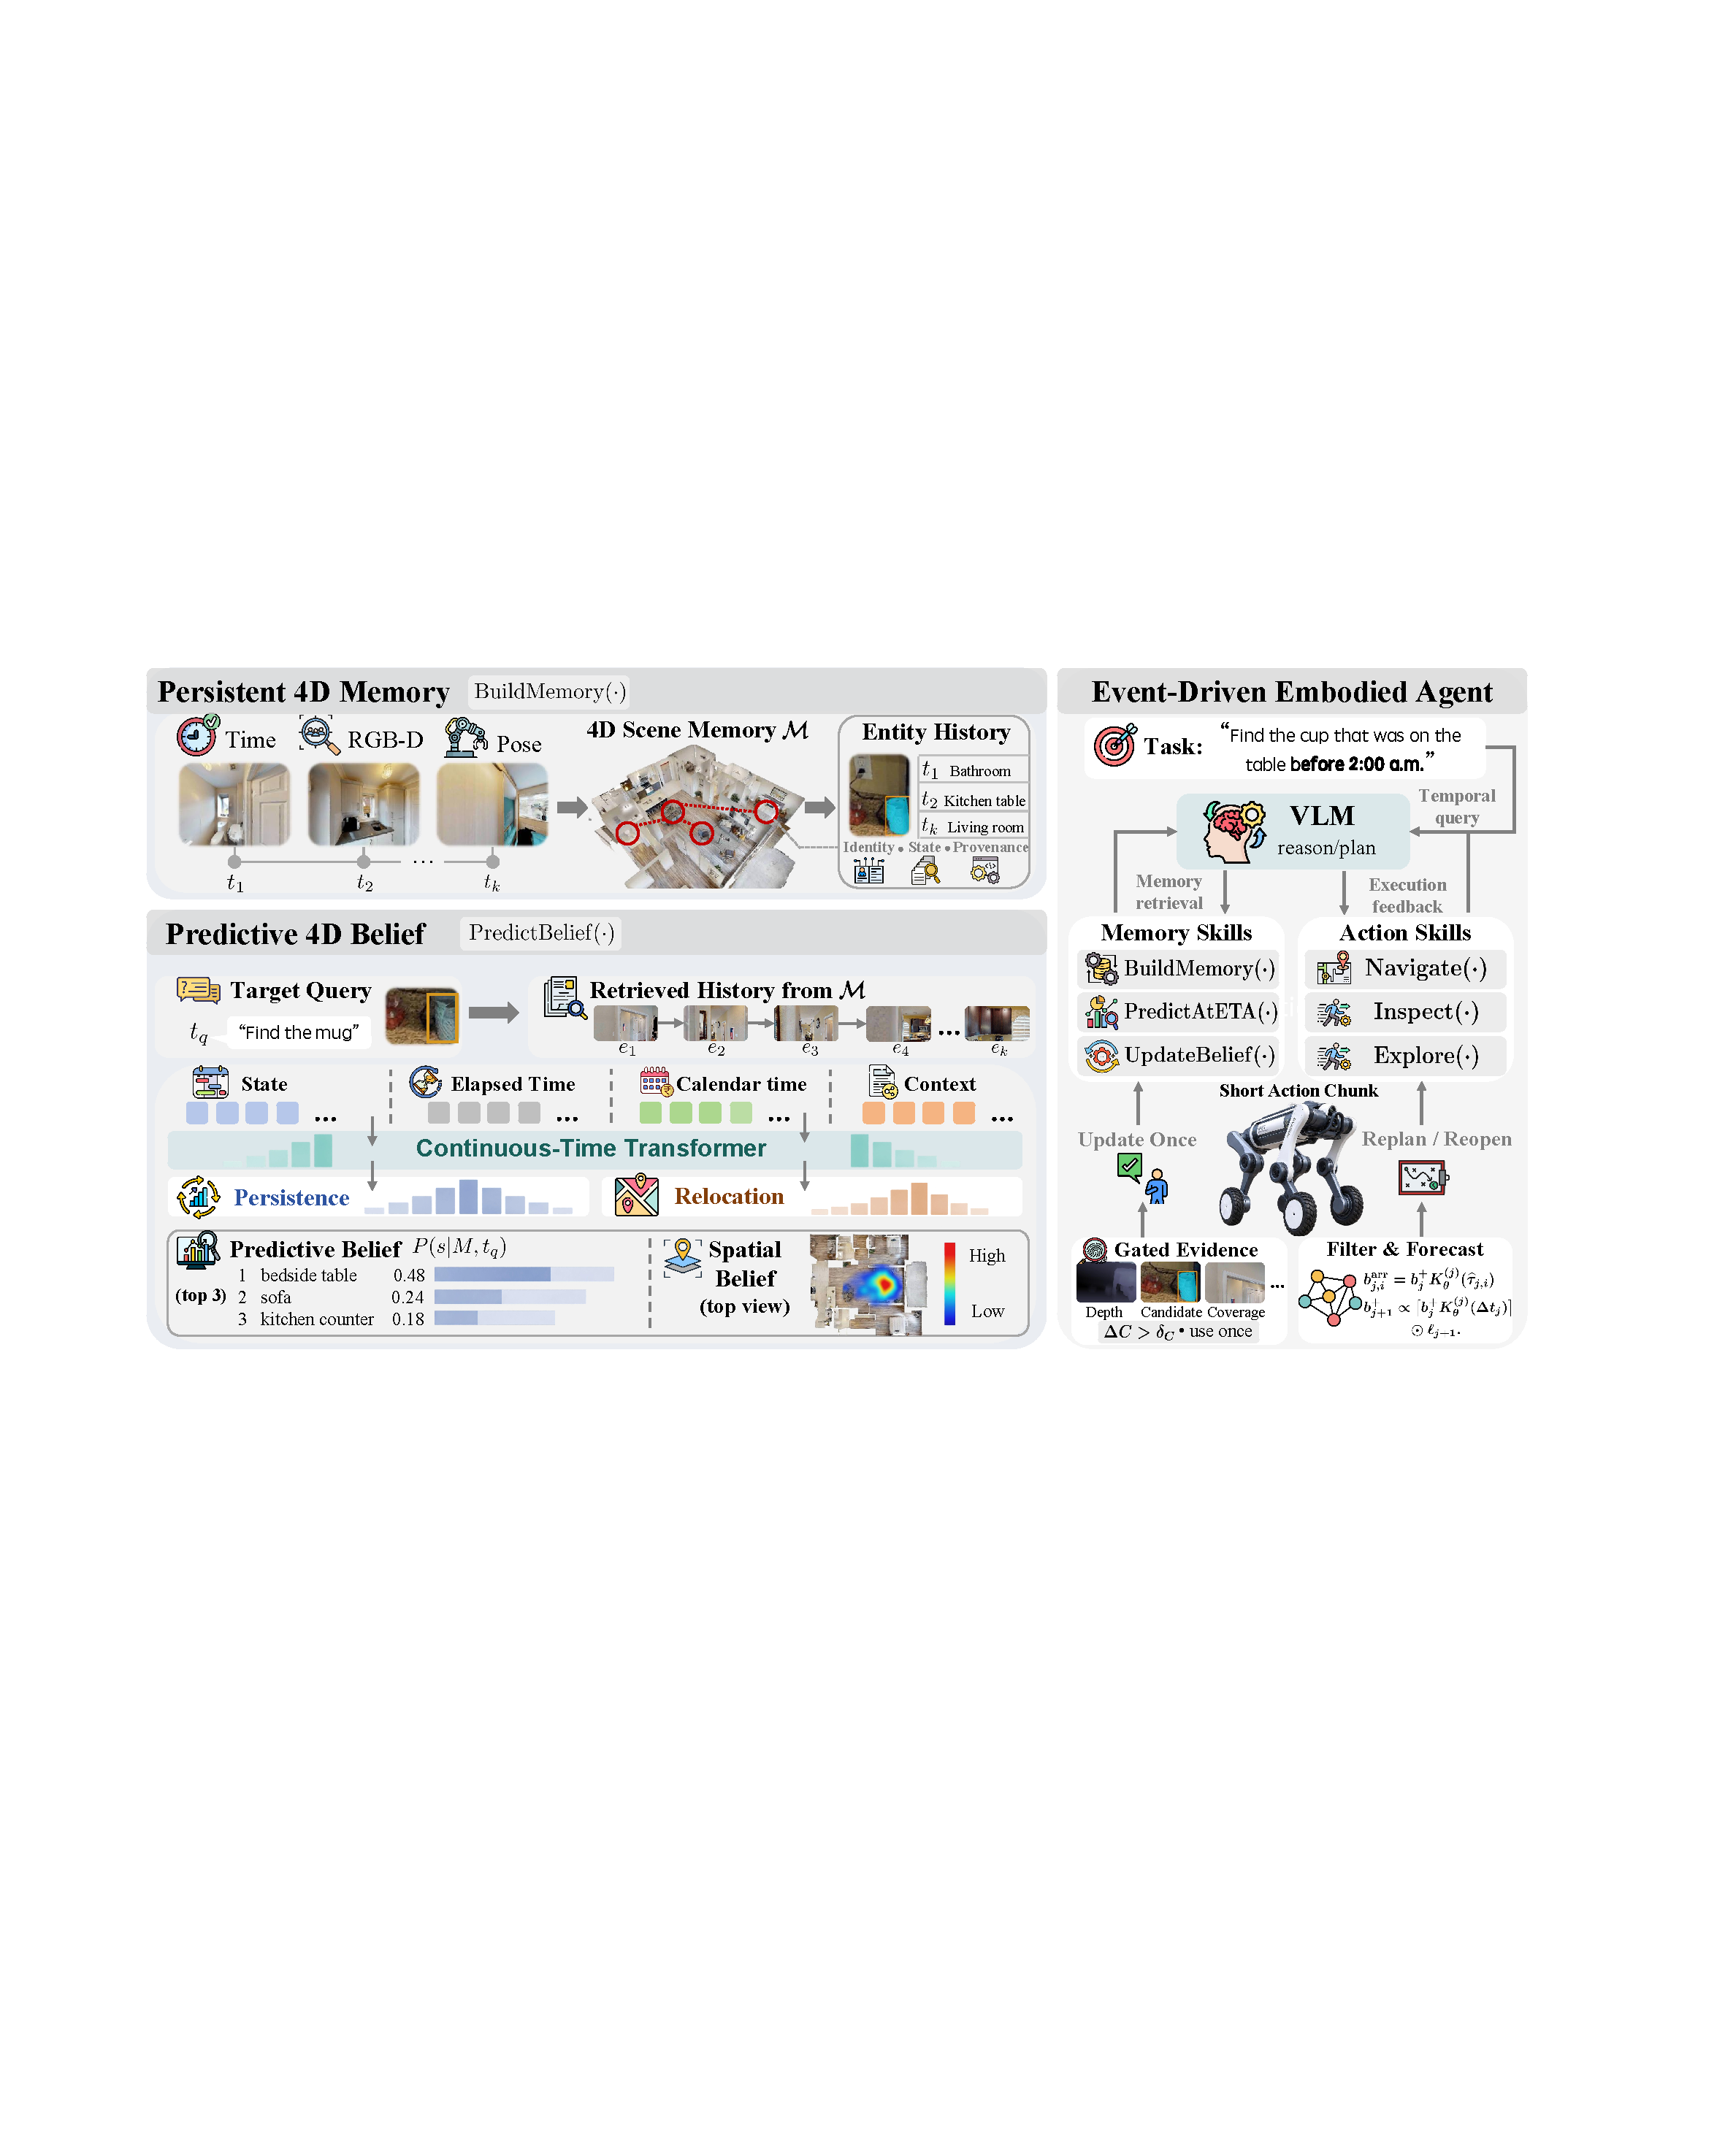
\includegraphics[width=\linewidth]{figures/method.pdf}
    \caption{\evolvingworldnav{} couples persistent 4D memory, predictive belief,
    and an embodied agent that updates and replans from stepwise evidence.}
    \label{fig:p4dnav_method}
\end{figure}

\subsection{Causal 4D Memory and History Encoding}
\label{sec:memory_encoding}
The 4D memory registers RGB-D observations in a shared frame, associates entities using
semantics, geometry, and time, and materializes versioned deltas causally:
\begin{equation}
\mathcal M_{\leq t}=\operatorname{Materialize}(\Delta\mathcal M_0,\ldots,\Delta\mathcal M_t)
=(\mathcal G_t,\mathcal V_t,\mathcal B_t),
\label{eq:memory}
\end{equation}
where $\mathcal G_t,\mathcal V_t,\mathcal B_t$ store relations, time-valid
versions, and provenance. Changes append versions without erasing history;
perception and versioning details are in \appref{app:memory-details}
\citep{liu2024grounding,ravi2025sam,radford2021learning}.

\paragraph{Target-conditioned history and continuous time.}
For target $o$, a typed query returns the most recent $K$ causal events
\begin{equation}
H_o=\{e_k=(o_k,s_k,t_k,z_k,c_k,v_k)\}_{k=1}^{K},
\label{eq:history}
\end{equation}
where $o_k,s_k,t_k,z_k$ encode entity, candidate state, time, and
$\{\mathrm{seen},\mathrm{notseen}\}$ evidence; $c_k,v_k$ encode confidence and
visibility. Related context events are causal, candidate encodings capture
function and geometry, and \texttt{unknown} absorbs unmapped states.

Each event token combines semantic, evidence, and temporal features:
\begin{align}
\mathbf x_k={}&E_o(o_k)+E_s(s_k)+E_z(z_k)+E_c(c_k)+E_v(v_k)\nonumber\\
&+\phi_{\Delta}(t_q-t_k)+\phi_{\mathrm{cal}}(t_k),
\label{eq:eventtoken}
\end{align}
where $\phi_{\Delta}$ encodes log elapsed time and $\phi_{\mathrm{cal}}$ encodes
hour and weekday. A query token specifies the target, time, and last observed state; a compact
Transformer yields
\begin{equation}
(\mathbf h_1,\ldots,\mathbf h_K,\mathbf h_q)
=\operatorname{CTTransformer}(\mathbf x_1,\ldots,\mathbf x_K,\mathbf x_q).
\label{eq:history-encoder}
\end{equation}
The encoding captures irregular intervals, evidence, and event order without hidden labels.

\subsection{Persistence--Relocation Belief}
\label{sec:belief_model}
We predict persistence at the last observed state or relocation elsewhere.
Episode validity guarantees a last positively observed state $s_{\mathrm{last}}$
(\appref{app:audit}). The persistence branch predicts
\begin{equation}
\rho_q=P(s_{t_q}^o=s_{\mathrm{last}}\mid H_o,t_q)
=\sigma(\mathbf w_{\rho}^{\top}\mathbf h_q).
\label{eq:persistence}
\end{equation}
For each alternative $i\in\widetilde{\mathcal C}_o\setminus
\{s_{\mathrm{last}}\}$, a shared pointer head computes
\begin{equation}
a_i=\frac{(W_q\mathbf h_q)^\top(W_c\mathbf g_i)}{\sqrt d}
+\psi(\mathbf h_q,\mathbf g_i),\qquad
\pi_q(i)=\frac{\exp a_i}{\sum_{u\in\widetilde{\mathcal C}_o\setminus\{s_{\mathrm{last}}\}}\exp a_u},
\label{eq:pointer}
\end{equation}
where $\mathbf g_i$ represents candidate $i$, $d$ is the projection dimension,
and $\psi$ measures learned compatibility. The prior is
\begin{equation}
b_q^-(i)=
\begin{cases}
\rho_q, & i=s_{\mathrm{last}},\\
(1-\rho_q)\pi_q(i), & i\neq s_{\mathrm{last}}.
\end{cases}
\label{eq:prior}
\end{equation}
We train with $\mathcal L_{\mathrm{state}}=-\log b_q^-(s_{t_q}^o)$ without
change labels; the normalized belief represents returns and alternatives.

\subsection{Predictive Embodied Agent}
\label{sec:agent}

A frozen VLM invokes memory, prediction, navigation, inspection, and exploration
tools. Action chunks, new coverage or evidence, ETA changes, and arrivals trigger
decision epochs. The encoder produces $\mathbf h_j$ for the row-normalized operator
\begin{equation}
[K_\theta^{(j)}(\Delta t)]_{r,u}=\operatorname{softmax}_{u}
f_\theta(\mathbf h_j,\mathbf g_r,\mathbf g_u,\phi_\Delta(\Delta t)).
\label{eq:transition-kernel}
\end{equation}
The operator shares the encoders in \cref{eq:history-encoder,eq:pointer}; a separate head
learns chronological state transitions through row-wise cross-entropy
(\appref{app:belief-control}). Initialized with $b_0^-=b_q^-$, the filter propagates after each chunk:
\begin{equation}
b_{j+1}^-=b_j^+K_\theta^{(j)}(t_{j+1}-t_j).
\label{eq:filter-predict}
\end{equation}
Thus $b_j^\pm$ denotes the current-time belief, separate from arrival forecasts.

\paragraph{Arrival-aware action selection.}
For candidate viewpoints $\mathcal W_i$, let
$d_{j,i}=d_{\mathrm{geo}}(x_j,\mathcal W_i)$ and $\widehat\tau_{j,i}$ be
the geodesic distance and estimated travel-plus-inspection time. The agent selects
\begin{equation}
i_j^*=\arg\max_{i\in\mathcal{C}_o}
\frac{
    p_{j,i}^{\mathrm{arr}}\,
    \widehat{q}_{j,i}^{\,\mathrm{new}}
}{
    d_{j,i}
    + \lambda_t \widehat{\tau}_{j,i}
    + \lambda_{\mathrm{inspect}}
},
\label{eq:planner}
\end{equation}
where $p_{j,i}^{\mathrm{arr}}$ is defined below and
$\widehat q_{j,i}^{\mathrm{new}}$ is the detection probability from newly covered
surfaces. Exploration expands the candidate set when unknown-state utility is highest.

\paragraph{Visibility-qualified measurement update.}
A posed RGB-D view can update every covered candidate. A calibrated detector estimates
$\widehat r_{j,i}=P(\mathrm{detect}\mid s_{t_j}=i,\mathbf f_{j,i})$ from
projected candidate geometry, online depth, and view features, without access to
ground-truth target masks or poses or simulator visibility flags. Given no detection,
\begin{equation}
\ell_j(i)=P(y_j=\varnothing\mid s_{t_j}=i)=
\begin{cases}
1-\widehat r_{j,i}, & i\in\mathcal C_o,\\
1, & i=\mathrm{unknown},
\end{cases}
\label{eq:negative}
\end{equation}
and the measurement posterior is
\begin{equation}
b_j^+(i)=\frac{b_j^-(i)\ell_j(i)}
{\sum_{u\in\widetilde{\mathcal C}_o}b_j^-(u)\ell_j(u)}.
\label{eq:bayes}
\end{equation}
An update uses only new surface coverage exceeding $\delta_C=0.05$, preventing
duplicate evidence from overlapping views. Dynamic reopening starts a new
time-valid round, allowing the same viewpoint to test a changed state. A verified match ends the search.

\paragraph{Posterior propagation and replanning.}
The current posterior is forecast to each candidate ETA for action selection,
without replacing the current-time filter:
\begin{equation}
b_{j,i}^{\mathrm{arr}}=b_j^+K_\theta^{(j)}(\widehat\tau_{j,i}),\qquad
p_{j,i}^{\mathrm{arr}}=b_{j,i}^{\mathrm{arr}}(i).
\label{eq:arrival-belief}
\end{equation}
Fixed-target episodes use identity dynamics; continuing evolution follows
\cref{eq:filter-predict,eq:arrival-belief}. At each epoch, the agent propagates
belief, incorporates new evidence once, forecasts arrival-time states, and replans
(\appref{app:belief-control}).
